\section{Current State}
In the current state, Willy is capable of autonomous movement, but if the previous group is to be believed, the current driving behaviour is reminiscent of "A drunken Pole".
This is obviously desirable, since WTR is meant to be a way of drawing in potential students with an interest in robotics and programming at Windesheim.
Having WTR be a danger to both the people around it and the walls/cupboards/any other furniture would be more likely to scare people away.

\subsection{Controlled Movement}
Before getting WTR driving autonomously, the movement is controlled using a Dualshock PS3 controller \cite{dualshock}.
While the \href{ https://windesheim-willy.github.io/WillyWiki/components/joystick.html}{Wiki} will claim that WTR can be controlled by holding the select button on the PS3 dualshock controller and moving the right joystick, in fact the left joystick needs to be used while holding down select.
Holding select means that the robot should essentially have a "dead-man's switch" \ref{trm::dms}.
Unfortunately, in the current state releasing select while having the joystick held in any direction causes WTR to continually repeat said movement, so if it is turning and the controller is accidentally dropped it will continue to turn in the direction is was heading.
This is obviously a dangerous oversight, and should be corrected ASAP.

\subsection{Autonomous Movement}
\todo{test autonomous movement}
\clearpage

\subsection{Rear Wheels Issues}
WTR is based of an old electric wheelchair/mobility scooter.
While this does provide a solid base that can carry a good amount of weight, it was never intended to drive by itself.
Steering is the biggest issue.
When WTR is simply driving in a straight line, (and the wheels are not being interfered with by the frame) it will do so properly.
The engines are mostly synchronised.
Issues arise when WTR is attempting to drive in a straight line after a turn.
Because the rear wheels are not motorized and turn on a pivot, they do not straighten themselves in any way, except for being dragged while driving straight.
This issue is illustrated in figure~\ref{fig::mvmnt}.

\begin{figure}[H]

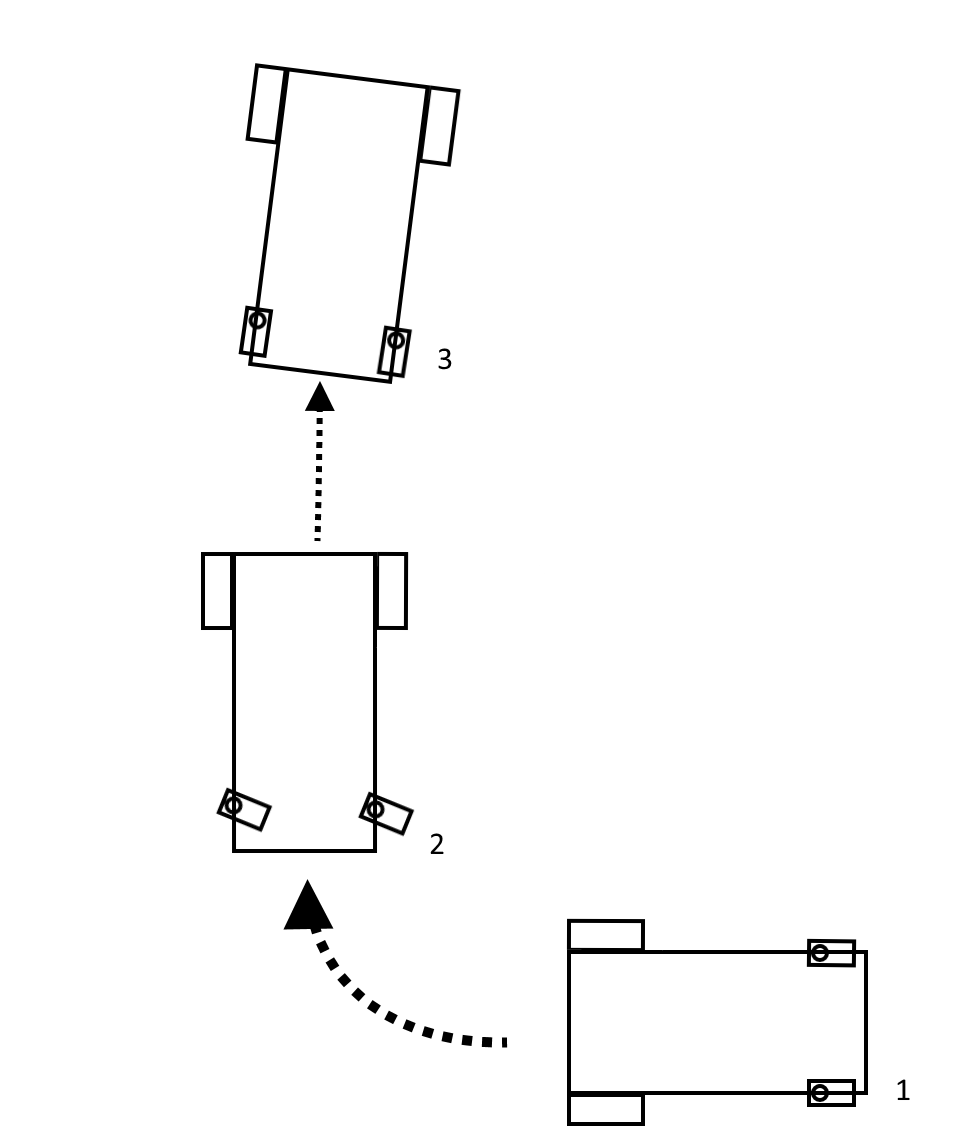
\includegraphics[width=10cm]{movementdiagram.png}
\caption{An approximation of the effect of the rear pivot wheels}
\label{fig::mvmnt}
\end{figure}
After driving for a meter or so, the wheels do straighten out, but because of the rotation made in straightening, they throw WTR off course.
As the wheels are not straightened while WTR is facing the desired direction, WTR when driving straight gets pulled to the side of the turn that was just made.
This can be compensated for in a few ways.

\begin{labeling}{Single Wheel Bearing}
\item [Tank Controls] By having both the front and rear wheels linked to the motor, steering happens around the center of the wheels, rather than the midpoint between the two frontal wheels. The downside of this is that it would require a compete rework of how WTR is made.
\item [Fixed Rear Wheels] By having the rear wheels have a fixed orientation, the issue of overshooting a turn becomes null, but it creates a new issue of necessitating a larger turning arc, which is counter-productive in a crowded environment.
\item [Single Wheel Bearing] Instead of having a rear wheel, a ball bearing which rolls along the ground and is attached to the frame by a fixture would completely remove all issues of getting the wheels stuck in a direction other than which WTR would need to move, but due to the weight of the frame WTR would have to carry this option is not realistic.
\item [Rotary Encoders] By adding rotary encoders to both the front and rear wheels, it would become possible to track the orientation of the rear wheels and the amount of rotations made by the front wheels. If this is known to WTR, then it can compensate for those issues. When the turn is finished, it can check how the rear wheels are positioned, and if they are not straight, drive in an arc towards its target until the wheels are properly oriented again. 
\end{labeling}

\newpage
